%!TEX root=report.tex
\subsection{Glacial Isostatic Adjustment}

The GRACE data that has been used in this report has not been corrected for Glacial Isostatic Adjustment (GIA), also called post-glacial rebound.

GIA is an real effect that makes land either rise, fall or shift horizontally. 
It can be observed at all locations which during the last ice age was covered by a thick layer of ice.
The cause is the sheer weight of the ice compressed the crust of the Earth so much, that when the ice retracted and the downward force was removed the crust started to rebound.
It is estimated that these movements will take many thousand years to subside.

\begin{figure}[H]
	\centering
	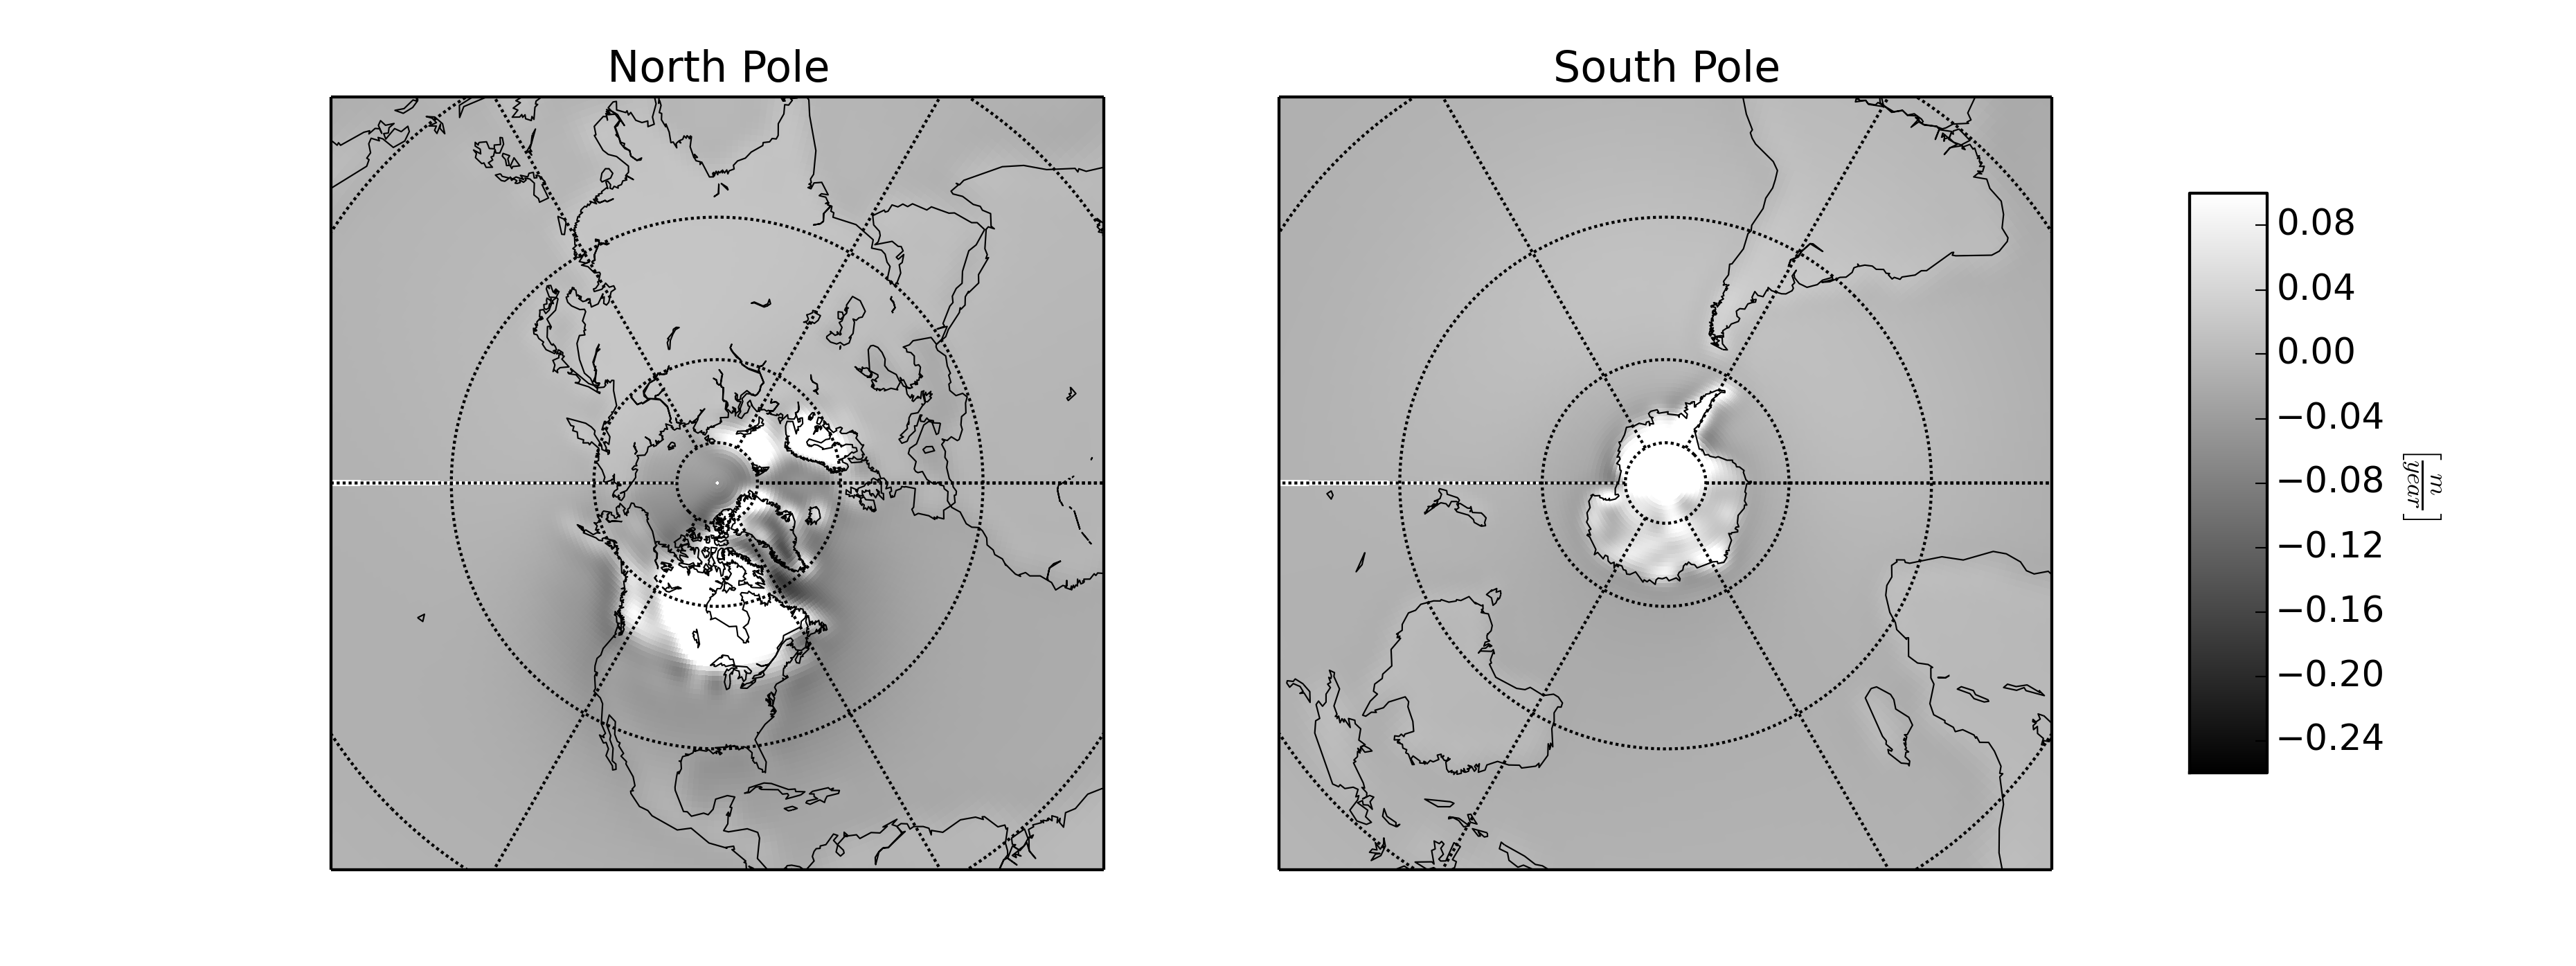
\includegraphics[width=\textwidth]{figures/gia-pure-adjust}
	\caption{Glacial Isostatic Adjustment. Data is based on ICE-5G and the specific source is NASA \cite{NASA-GIA-download}.}
	\label{fig:gia-pure-adjust}
\end{figure}

The GRACE data just measures the gravity and because this effect is real the rebound should be observed here.
Thus one can not directly conclude from the GRACE data, if changes are caused by recent ice melting or GIA. Removing the GIA signal is therefor important, if one which to make conclusion about ice melting caused by climatic changes.

\begin{figure}[H]
	\centering
	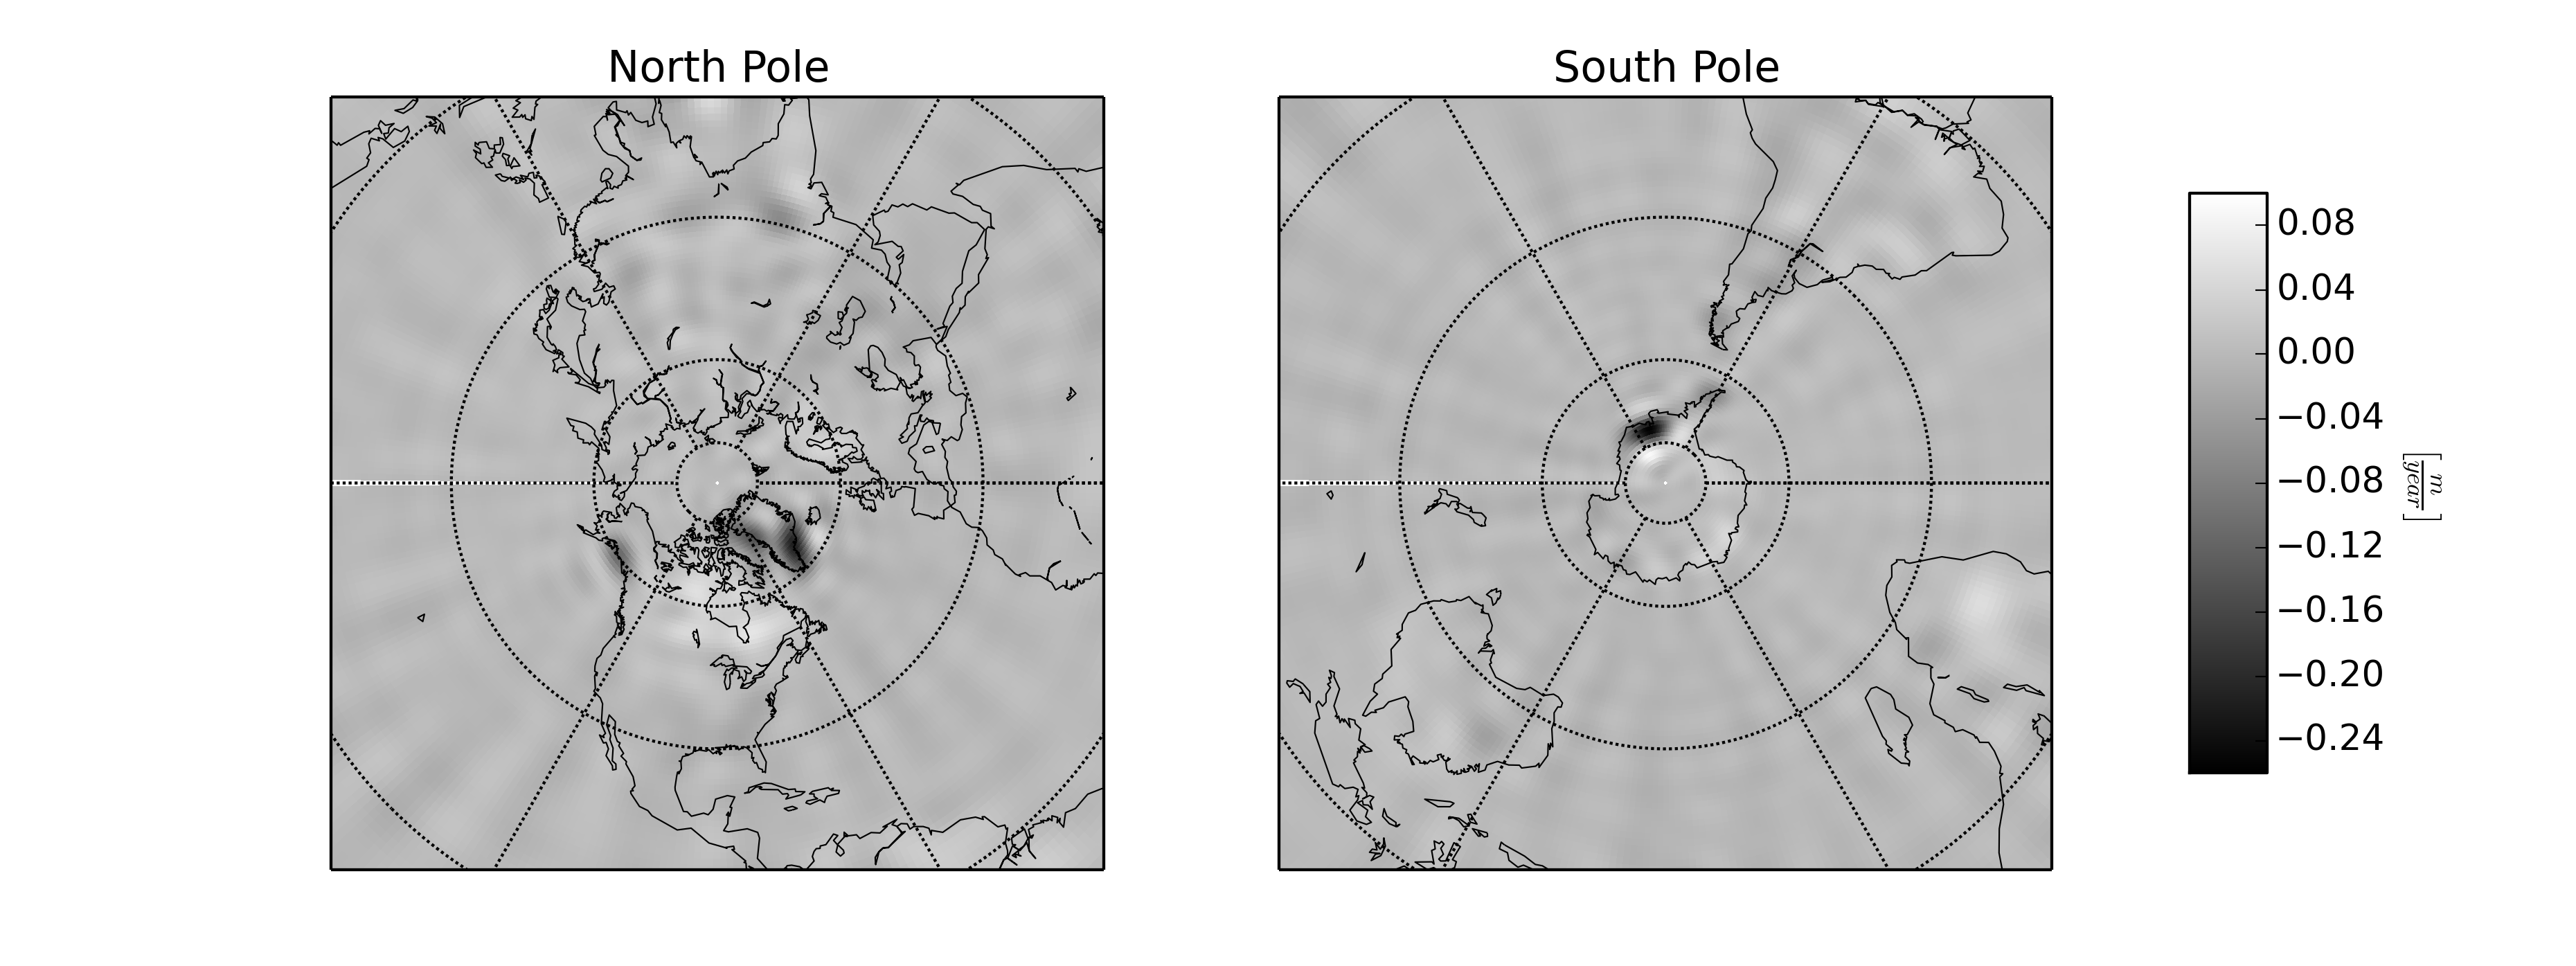
\includegraphics[width=\textwidth]{figures/gia-just-vel}
	\caption{Estiamted velocity from GRACE data, without correction for GIA.}
	\label{fig:gia-just-vel}
\end{figure}

\begin{figure}[H]
	\centering
	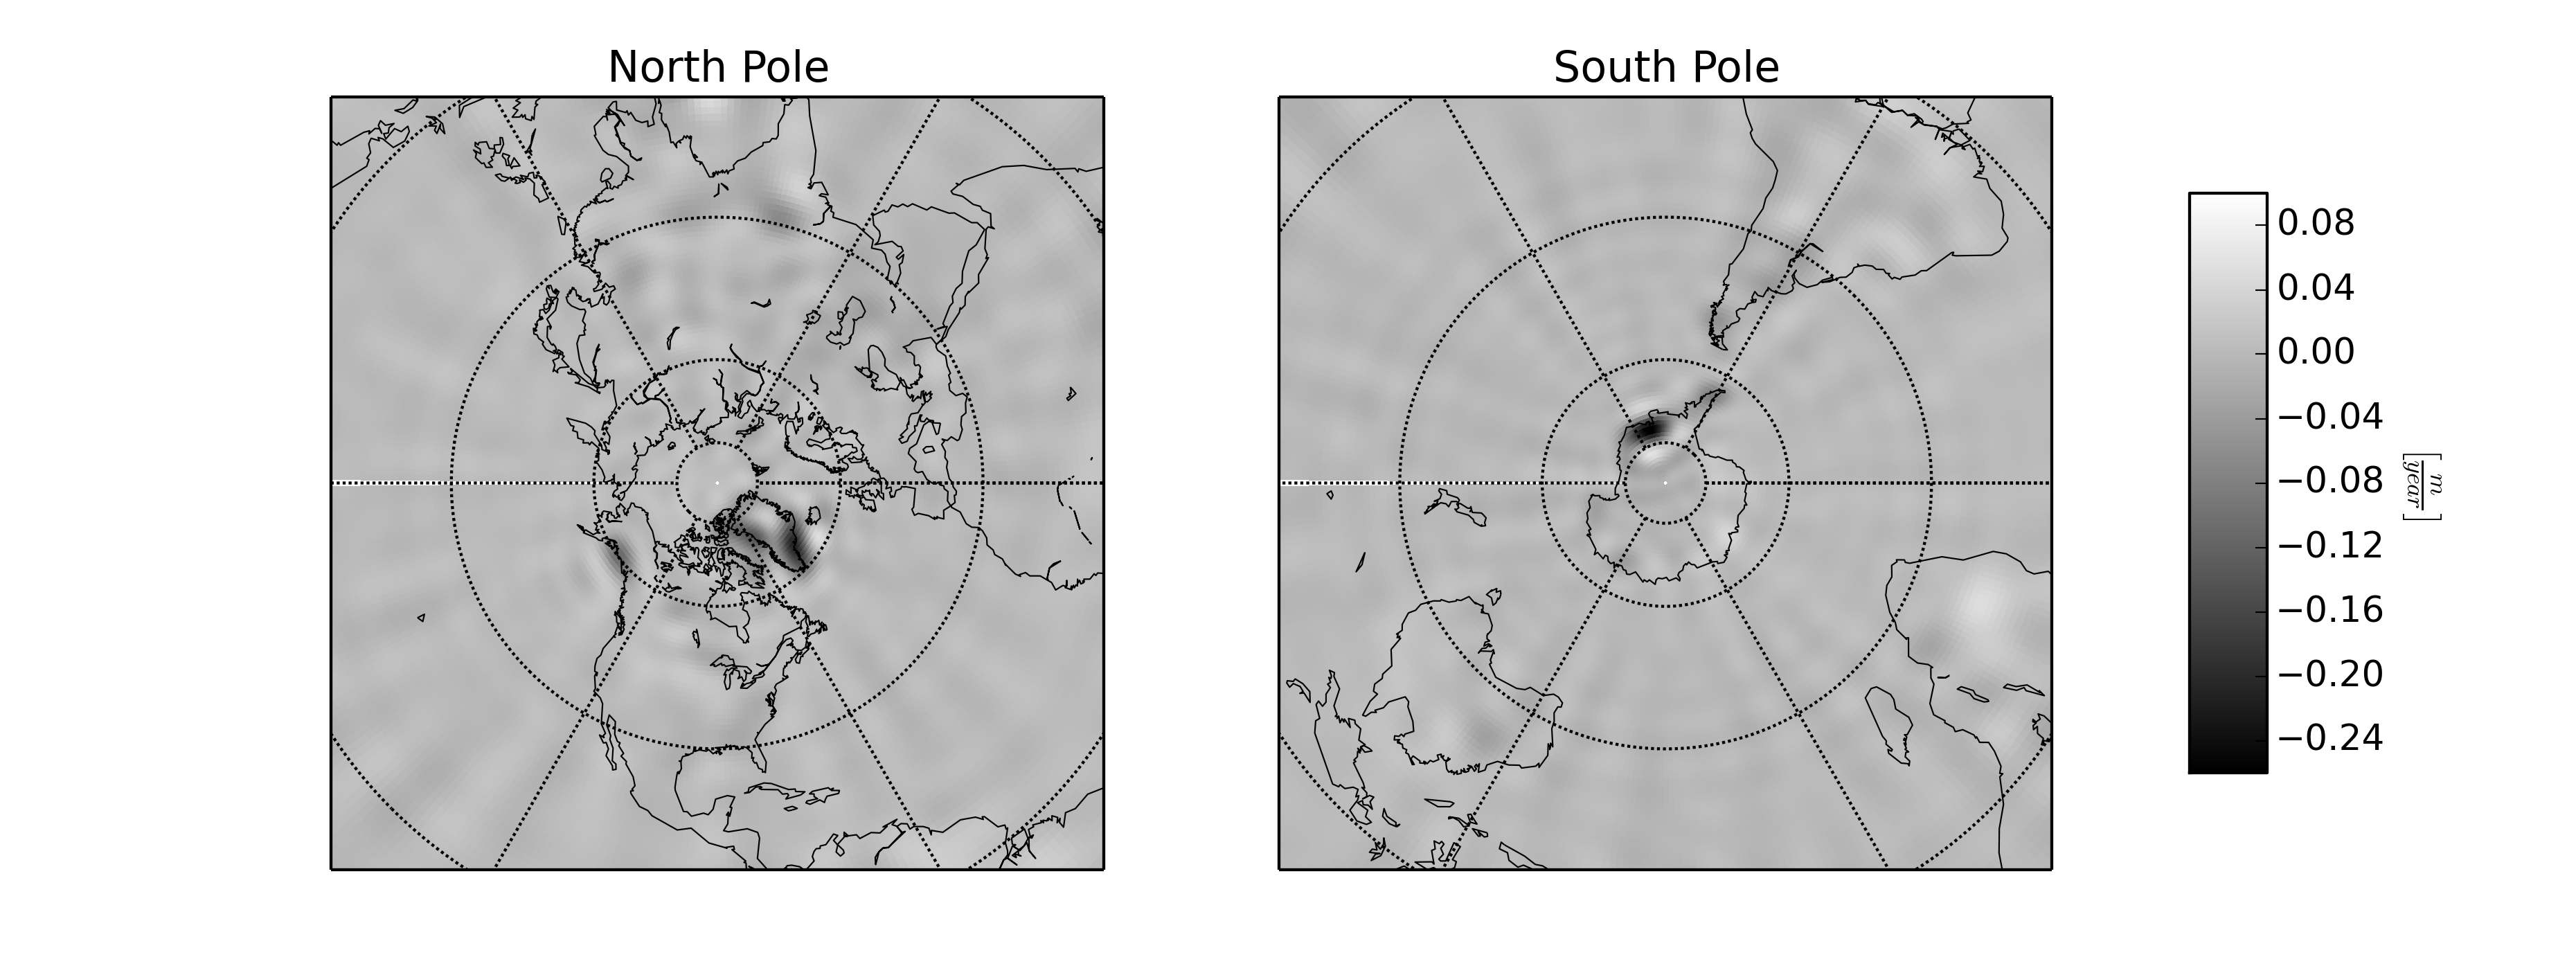
\includegraphics[width=\textwidth]{figures/gia-adjust-vel}
	\caption{Estiamted velocity from GRACE data, with the GIA signal removed. A big improvement around North America can be observed.}
	\label{fig:gia-adjust-vel}
\end{figure}

Even though there appears to be a significant velocity in EWH after GIA have been removed from the velocity estimate, one still have to be careful about making conclusions. According to NASA \cite{NASA-GIA-incomplete}, in order to sufficiently correct for GIA, region specific averaging kernels are needed to properly account for GIA as well as noise from nearby land hydrology.

NASA specifically state \cite{NASA-GIA-incomplete} that the GRACE data (with standard GIA applied) is not suited for Cryospheric studies (ice mass changes) and thus one should keep these reservations in mind when viewing the results.

\textit{For the remaining report no correction for GIA have been used. Only this section have the standard GIA correction.}
